\documentclass[../main.tex]{subfiles}

\begin{document}
\subsection{Implementation Plan}
TrackMe system is composed of five macro components (\textit{fig. 2}) that can be developed independently and simultanously
after interfaces and communications standards are properly choosen.\\



\subsection{Integration Plan}
Although macro components will be developed indipendently, it is strongly suggested a top-down approach oriented toward functionalities
implementation. 
 \subsubsection{Mobile Client, Applications and Database Servers}
    The first thing to be developed will be the "core functionality of the system" and Data4Help (\textit{Fig. 9}). Then it will be possible
    to test the backbone of the system (servers communication, models and APIs). Following the same approach, the development will focus consequently on
    AutomatedSOS and then on Track4Run.

    \begin{figure}[ht]
        \centering
             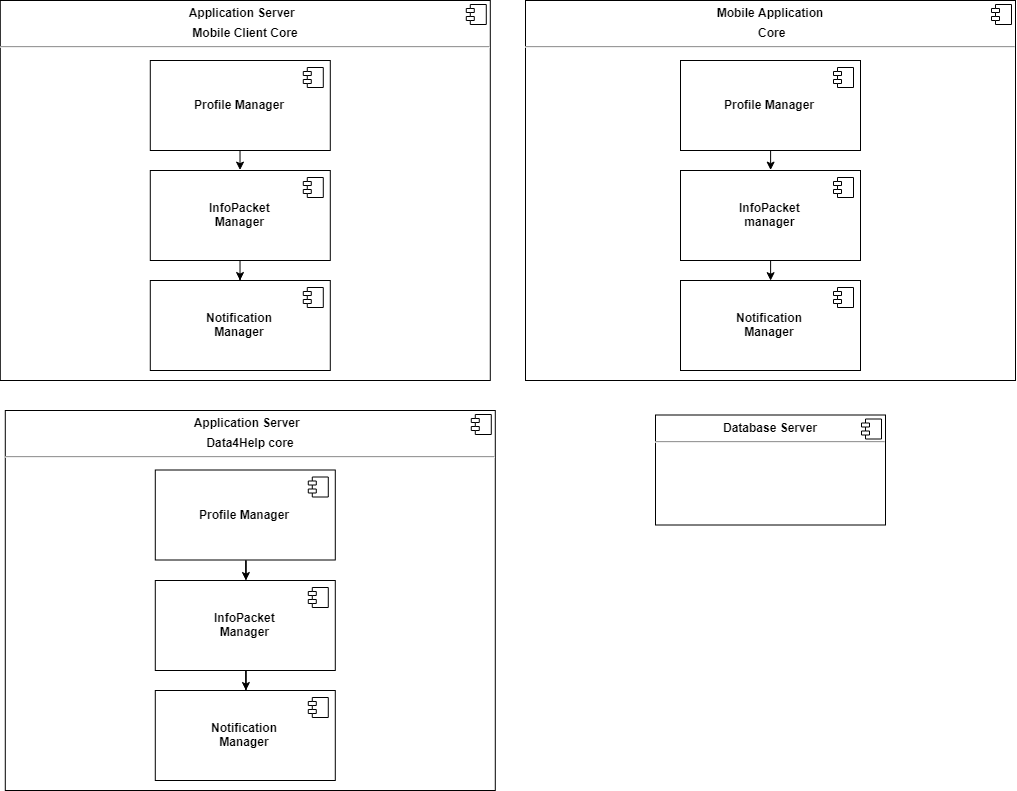
\includegraphics[width=1.0\textwidth]{development.png}
              \caption{core functionality development}
               \label{fig:development}
    \end{figure}
 \subsubsection{Web Server}
    Being a totally independent part of the system, the Web Server will be developed by a different team or after the development of the other components.\\
    The APIs documentation to be hosted on the Web Server will be produced by the Data4Help Application server developers. 
\subsection{Test Plan}
    Following the top-down approach, each module should be tested as soon as it is completed.
\subsubsection{System Testing}
    The application will be firstly beta tested in the urban area of Milan, thus it will be possible
    to gather statistics about application usage and user base to better plan a final release.\\
    The system must be able to withstand constant data upload from our users devices. The mobile application servers must be backed up
    by another server that guarantee at least AutomatedSOS availability 24/7 in case of failure.\\
    We expect companies to make a large volume of request to Data4Help server, so it should be subject to load and stress tests.
 
\end{document}
